% 图 76.3 —— 由 `checks/emit_hand.py` 自动拼出（probe 精测 + prims2 图元分解）
%%
% ⚠ 这是**稿子不是成品**：跑 `checks/checkhand.py 76.3` 看指标 + 看叠合图。
%%
%% ⚠ 待核：
%   · 本图 probe 报出阴影族 1 个 —— **本脚本不生成阴影**（要照原书手写）；prims2 的 strokes 里可能含阴影线，核对时留意别画重
%   · 可疑字形 1 项（空心圈 ⊙ 常被认成字母 o）—— 见文件末
%%
\documentclass[12pt]{standalone}
\usepackage{fontspec}
\setsansfont{Arial}
\newfontfamily\mfallback{DejaVu Sans}
\usepackage{tikz}
\usetikzlibrary{arrows.meta}
\begin{document}
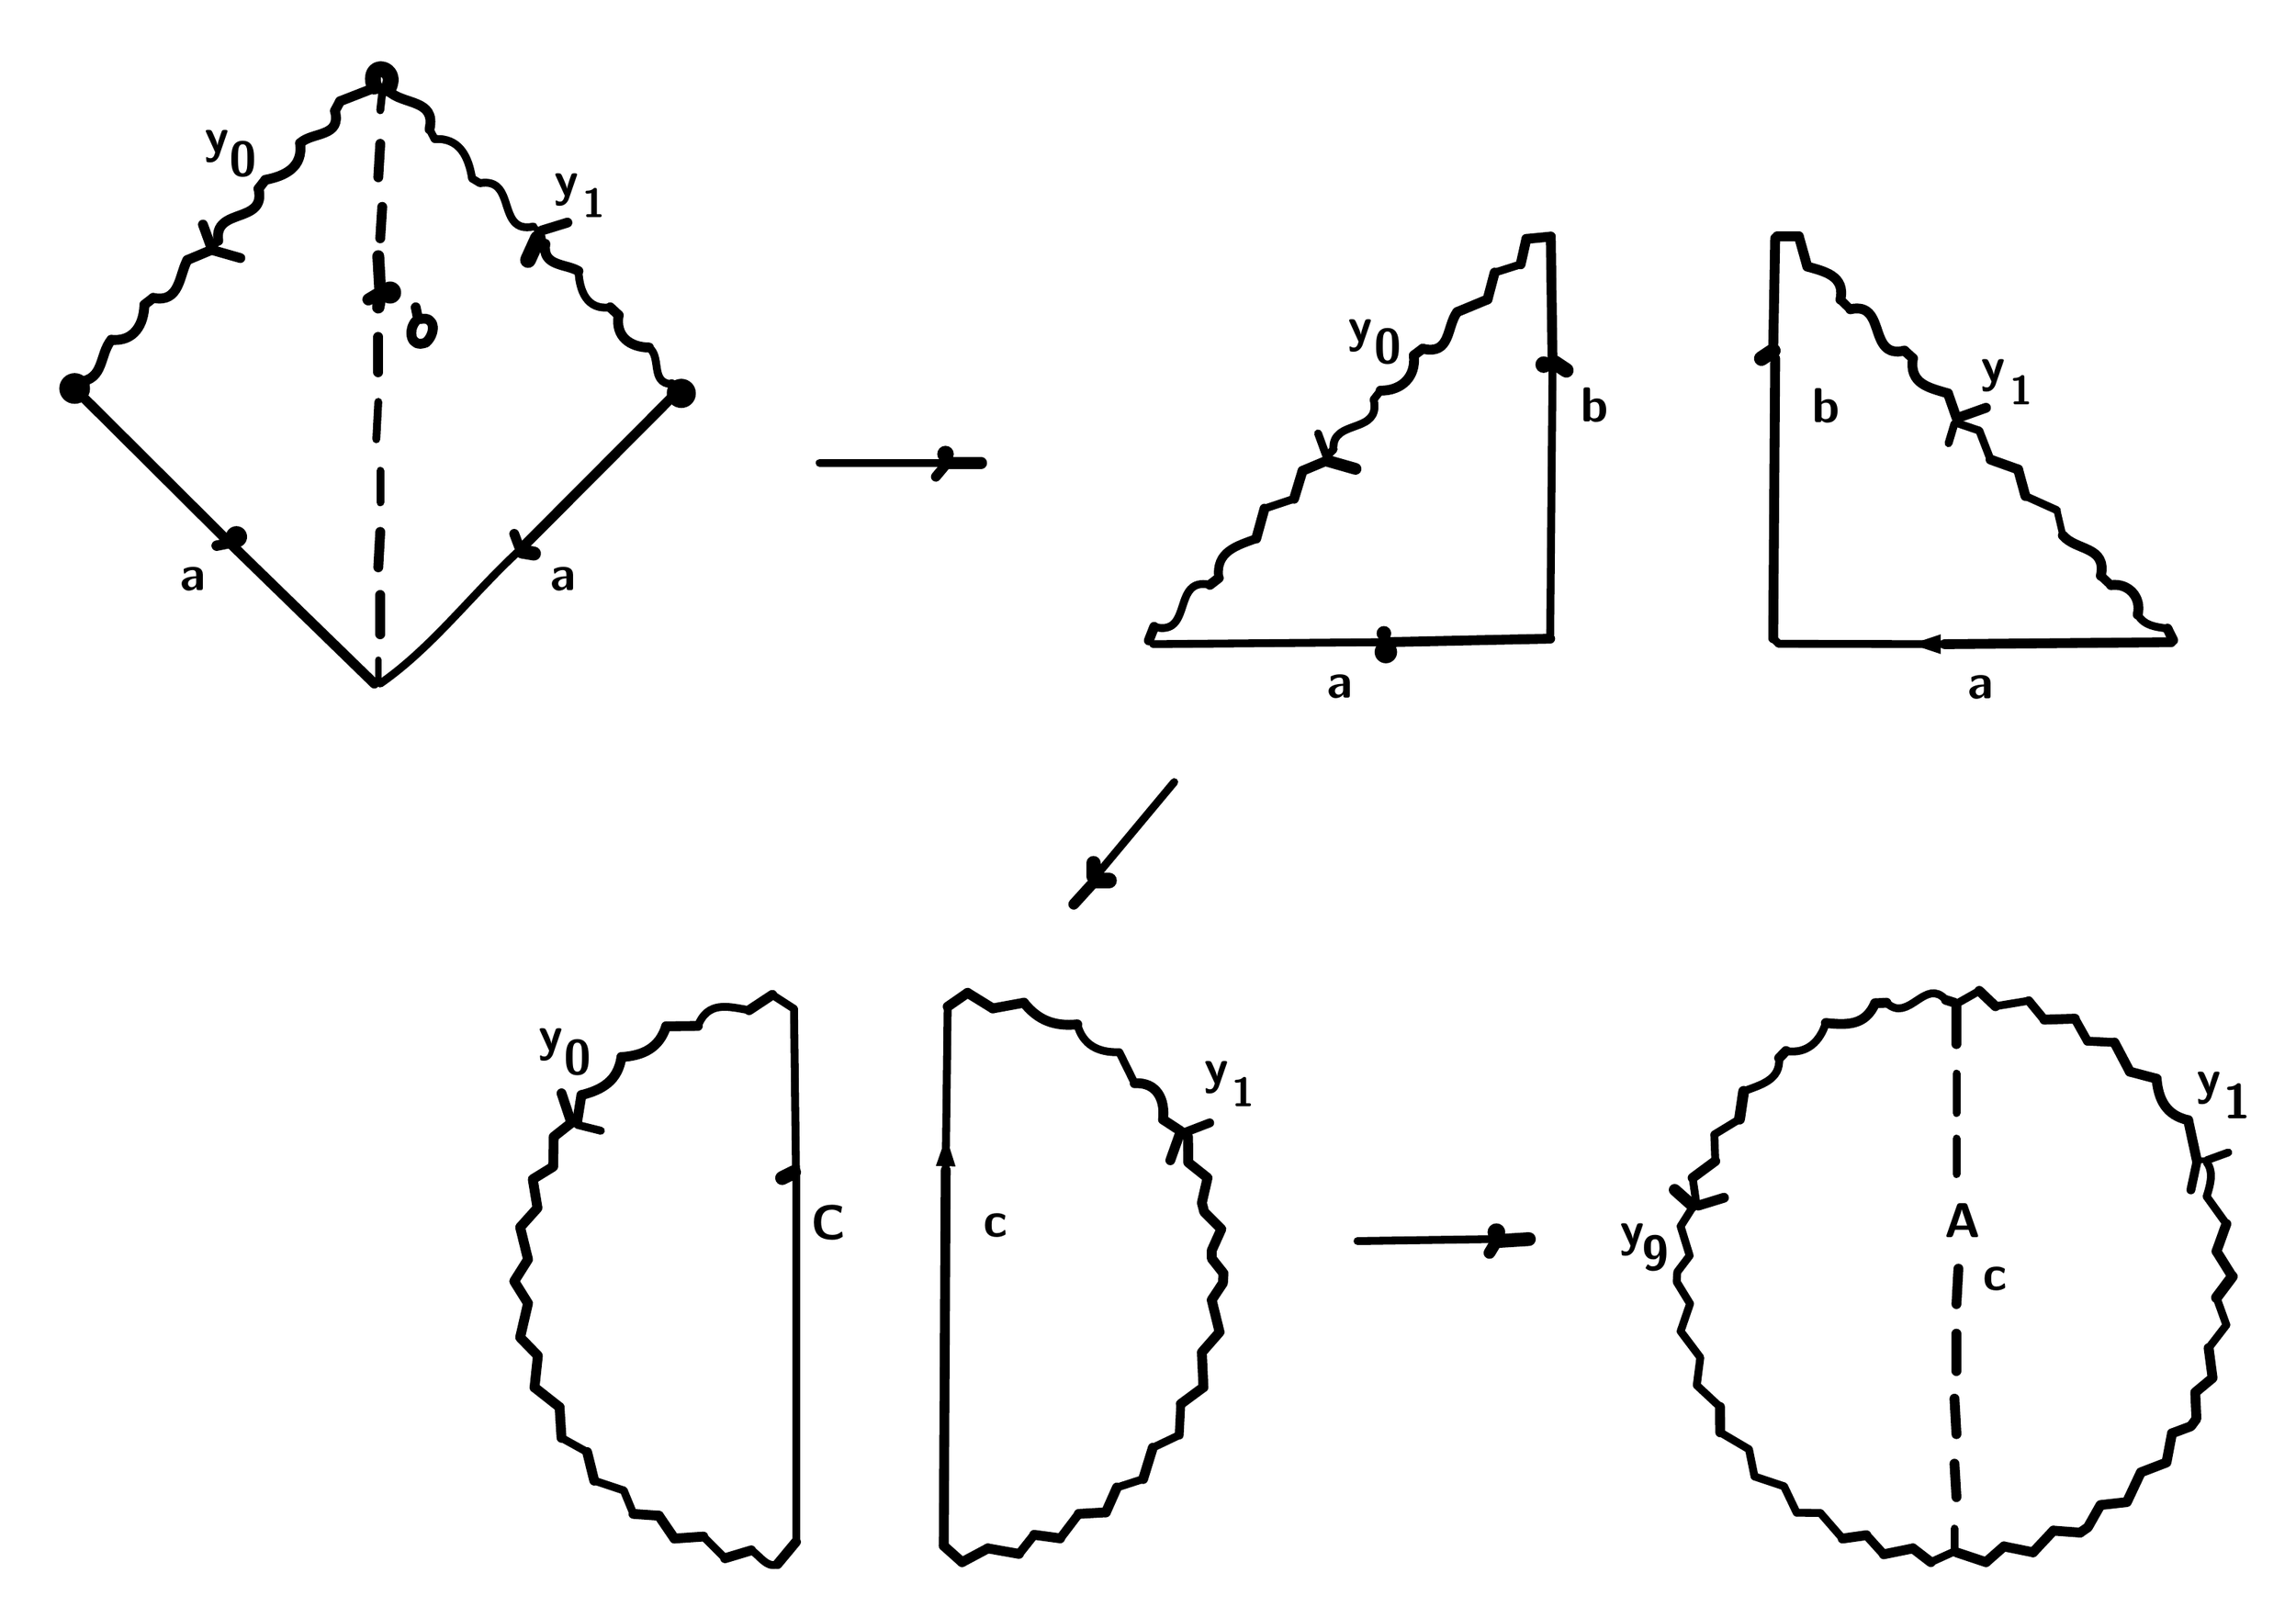
\begin{tikzpicture}[x=1pt, y=-1pt, line width=4.0pt, line cap=round, line join=round]

  %% ════ 填充区（prims2 的 fills）════

  %% ════ 直线段（prims2 的 strokes）════
  \draw[line width=4.0pt] (663.0,221.0) -- (659.0,210.0);
  \draw[line width=6.0pt] (849.0,602.0) -- (840.0,594.0);
  \draw[line width=5.0pt] (998.0,197.0) -- (984.0,202.0);
  \draw[line width=5.0pt] (470.0,226.0) -- (465.0,232.0);
  \draw[line width=6.0pt] (183.0,138.0) -- (182.0,120.0);
  \draw[line width=5.0pt] (112.0,121.0) -- (98.0,117.0);
  \draw[line width=4.0pt] (283.0,561.0) -- (295.0,564.0);
  \draw[line width=5.0pt] (778.0,173.0) -- (777.1,110.1);
  \draw[line width=5.0pt] (777.1,110.1) -- (764.7,111.3);
  \draw[line width=5.0pt] (764.7,111.3) -- (761.8,124.2);
  \draw[line width=4.0pt] (761.8,124.2) -- (748.6,128.4);
  \draw[line width=5.0pt] (748.6,128.4) -- (745.0,142.0);
  \draw[line width=5.0pt] (745.0,142.0) -- (729.6,148.4);
  \draw[line width=5.0pt] (712.1,167.0) -- (707.6,170.4);
  \draw[line width=4.0pt] (690.7,188.3) -- (687.2,192.8);
  \draw[line width=4.0pt] (666.8,218.2) -- (664.0,221.0);
  \draw[line width=4.0pt] (1121.0,575.0) -- (1110.0,579.0);
  % （略）线段 (469.0,583.0)-(464.0,586.0) 线宽6.1 —— 是箭头头那一坨，已由箭头头代替
  \draw[line width=5.0pt] (179.0,35.0) -- (162.6,41.4);
  \draw[line width=5.0pt] (162.6,41.4) -- (160.0,46.3);
  \draw[line width=5.0pt] (124.7,81.3) -- (121.2,85.8);
  \draw[line width=4.0pt] (100.8,112.2) -- (98.0,115.0);
  \draw[line width=4.9pt] (982.0,499.0) -- (977.6,497.6);
  \draw[line width=5.0pt] (947.5,499.0) -- (941.7,499.3);
  \draw[line width=5.0pt] (896.5,523.5) -- (893.0,527.1);
  \draw[line width=5.5pt] (875.0,544.0) -- (872.9,558.1);
  \draw[line width=4.0pt] (872.9,558.1) -- (860.1,565.9);
  \draw[line width=4.0pt] (860.1,565.9) -- (860.6,579.4);
  \draw[line width=5.0pt] (860.6,579.4) -- (849.1,587.9);
  \draw[line width=4.0pt] (849.1,587.9) -- (851.0,601.0);
  \draw[line width=5.0pt] (1092.0,316.0) -- (977.0,317.0);
  \draw[line width=6.0pt] (471.0,225.0) -- (488.0,225.0);
  \draw[line width=4.0pt] (984.0,205.0) -- (994.6,208.6);
  \draw[line width=4.0pt] (994.6,208.6) -- (1000.3,223.3);
  \draw[line width=5.0pt] (1000.3,223.3) -- (1014.3,228.3);
  \draw[line width=5.0pt] (1014.3,228.3) -- (1018.0,241.8);
  \draw[line width=4.0pt] (1018.0,241.8) -- (1034.0,249.0);
  \draw[line width=3.5pt] (1034.0,249.0) -- (1037.0,261.8);
  \draw[line width=4.5pt] (1056.3,282.3) -- (1061.4,287.0);
  \draw[line width=5.0pt] (1090.1,309.1) -- (1093.0,315.0);
  \draw[line width=7.4pt] (779.0,174.0) -- (785.0,178.0);
  \draw[line width=4.0pt] (470.0,582.0) -- (471.0,501.0);
  \fill (475.0,582.1) -- (465.0,581.9) -- (470.2,567.0) -- cycle;
  \draw[line width=5.0pt] (471.0,501.0) -- (481.1,494.0);
  \draw[line width=5.0pt] (481.1,494.0) -- (493.9,501.9);
  \draw[line width=5.0pt] (493.9,501.9) -- (509.7,499.0);
  \draw[line width=4.0pt] (558.1,524.1) -- (565.9,539.9);
  \draw[line width=5.0pt] (580.3,558.3) -- (589.0,564.0);
  \draw[line width=5.0pt] (183.0,111.0) -- (184.0,95.0);
  \draw[line width=5.0pt] (983.0,500.0) -- (983.0,520.0);
  \draw[line width=4.5pt] (591.0,565.0) -- (604.0,560.0);
  \draw[line width=5.0pt] (591.0,565.0) -- (593.0,567.2) -- (593.1,580.1) -- (602.9,587.9) -- (600.0,600.6) -- (601.2,605.2) -- (609.9,613.9) -- (605.0,624.8) -- (605.0,628.8) -- (611.0,636.4) -- (610.7,641.3) -- (605.0,649.9) -- (609.0,666.2) -- (600.0,676.5) -- (600.8,694.2);
  \draw[line width=5.0pt] (600.8,694.2) -- (589.3,702.7);
  \draw[line width=4.5pt] (589.3,702.7) -- (588.5,718.5);
  \draw[line width=4.0pt] (588.5,718.5) -- (575.1,724.9);
  \draw[line width=5.0pt] (575.1,724.9) -- (570.2,740.8);
  \draw[line width=4.0pt] (570.2,740.8) -- (556.9,745.1);
  \draw[line width=5.0pt] (556.9,745.1) -- (551.3,757.7);
  \draw[line width=5.0pt] (551.3,757.7) -- (537.5,758.5);
  \draw[line width=4.5pt] (537.5,758.5) -- (528.1,770.9);
  \draw[line width=5.0pt] (528.1,770.9) -- (514.9,769.1);
  \draw[line width=4.5pt] (514.9,769.1) -- (507.2,778.8);
  \draw[line width=5.0pt] (507.2,778.8) -- (491.4,776.0);
  \draw[line width=5.0pt] (491.4,776.0) -- (478.3,783.0);
  \draw[line width=5.0pt] (478.3,783.0) -- (469.0,774.7);
  \draw[line width=5.0pt] (469.0,774.7) -- (470.0,584.0);
  \draw[line width=4.0pt] (983.0,555.0) -- (983.0,535.0);
  \draw[line width=5.5pt] (535.0,449.0) -- (545.0,438.0);
  % （略）线段 (471.0,583.0)-(476.0,587.0) 线宽6.5 —— 是箭头头那一坨，已由箭头头代替
  \draw[line width=4.0pt] (984.0,499.0) -- (994.6,493.0);
  \draw[line width=5.0pt] (994.6,493.0) -- (1002.8,500.8);
  \draw[line width=4.0pt] (1002.8,500.8) -- (1019.7,498.0);
  \draw[line width=4.5pt] (1019.7,498.0) -- (1027.6,507.6);
  \draw[line width=5.0pt] (1027.6,507.6) -- (1043.1,507.1);
  \draw[line width=4.5pt] (1043.1,507.1) -- (1049.5,518.5);
  \draw[line width=4.5pt] (1049.5,518.5) -- (1063.2,519.2);
  \draw[line width=5.0pt] (1063.2,519.2) -- (1071.0,534.0);
  \draw[line width=5.0pt] (1071.0,534.0) -- (1084.6,537.6);
  \draw[line width=5.0pt] (1100.6,558.6) -- (1105.0,579.0);
  \draw[line width=4.0pt] (849.0,603.0) -- (843.0,612.5) -- (847.6,627.4) -- (841.3,635.7) -- (841.0,640.7) -- (847.8,651.8) -- (843.0,665.8) -- (853.0,679.1) -- (851.2,693.2);
  \draw[line width=4.0pt] (851.2,693.2) -- (863.0,704.2);
  \draw[line width=5.0pt] (863.0,704.2) -- (863.1,717.1);
  \draw[line width=4.0pt] (863.1,717.1) -- (877.7,725.7);
  \draw[line width=4.0pt] (877.7,725.7) -- (880.5,739.5);
  \draw[line width=4.0pt] (880.5,739.5) -- (895.5,744.5);
  \draw[line width=4.0pt] (895.5,744.5) -- (901.9,757.9);
  \draw[line width=4.0pt] (901.9,757.9) -- (913.9,758.0);
  \draw[line width=4.0pt] (913.9,758.0) -- (925.2,771.0);
  \draw[line width=5.0pt] (925.2,771.0) -- (937.3,769.3);
  \draw[line width=4.5pt] (937.3,769.3) -- (946.1,779.0);
  \draw[line width=5.0pt] (946.1,779.0) -- (960.9,776.0);
  \draw[line width=5.0pt] (960.9,776.0) -- (970.0,783.0);
  \draw[line width=4.0pt] (970.0,783.0) -- (981.0,778.0);
  \draw[line width=5.0pt] (280.0,560.0) -- (275.0,545.0);
  \draw[line width=5.0pt] (280.0,560.0) -- (271.0,567.1) -- (270.8,582.2) -- (260.4,588.6) -- (262.8,603.2) -- (254.0,613.0) -- (258.0,629.3) -- (251.0,640.4) -- (258.0,651.6) -- (254.0,668.9) -- (263.0,678.2) -- (261.3,694.3);
  \draw[line width=5.0pt] (261.3,694.3) -- (274.0,704.3);
  \draw[line width=5.0pt] (274.0,704.3) -- (275.0,719.9);
  \draw[line width=4.0pt] (275.0,719.9) -- (288.0,727.1);
  \draw[line width=5.0pt] (288.0,727.1) -- (291.6,741.6);
  \draw[line width=4.0pt] (291.6,741.6) -- (306.6,746.6);
  \draw[line width=4.0pt] (306.6,746.6) -- (311.5,758.5);
  \draw[line width=5.0pt] (311.5,758.5) -- (324.4,759.4);
  \draw[line width=5.0pt] (324.4,759.4) -- (332.3,771.0);
  \draw[line width=5.0pt] (332.3,771.0) -- (347.0,770.0);
  \draw[line width=4.0pt] (347.0,770.0) -- (358.0,781.0);
  \draw[line width=5.0pt] (358.0,781.0) -- (371.3,777.0);
  \draw[line width=5.0pt] (384.6,784.0) -- (394.0,772.7);
  \draw[line width=4.0pt] (394.0,772.7) -- (394.0,587.0);
  \draw[line width=4.0pt] (983.0,568.0) -- (983.0,586.0);
  \draw[line width=5.0pt] (106.0,265.0) -- (29.0,188.4);
  \draw[line width=4.8pt] (29.0,188.4) -- (30.2,183.8);
  \draw[line width=5.0pt] (63.3,144.7) -- (67.8,141.2);
  \draw[line width=5.0pt] (85.1,122.0) -- (97.0,117.0);
  \draw[line width=5.0pt] (183.0,260.0) -- (182.0,278.0);
  \draw[line width=4.5pt] (1102.0,594.0) -- (1105.0,580.0);
  \draw[line width=4.0pt] (181.0,213.0) -- (182.0,194.0);
  \draw[line width=5.0pt] (982.0,733.0) -- (983.0,750.0);
  \draw[line width=6.0pt] (746.0,626.0) -- (749.0,621.0);
  \draw[line width=6.3pt] (182.0,146.0) -- (183.0,140.0);
  \draw[line width=5.0pt] (182.0,161.0) -- (182.0,179.0);
  \draw[line width=5.0pt] (283.0,559.0) -- (285.1,545.9);
  \draw[line width=5.0pt] (328.1,511.0) -- (344.2,510.8);
  \draw[line width=5.0pt] (370.2,502.8) -- (382.0,495.0);
  \draw[line width=4.0pt] (382.0,495.0) -- (393.0,502.1);
  \draw[line width=4.0pt] (393.0,502.1) -- (394.0,584.0);
  \draw[line width=4.0pt] (208.0,55.6) -- (210.6,60.6);
  \draw[line width=4.0pt] (229.6,80.6) -- (233.6,83.0);
  \draw[line width=3.0pt] (260.8,105.0) -- (263.0,107.0);
  \draw[line width=8.0pt] (263.0,111.0) -- (258.0,122.0);
  \draw[line width=3.0pt] (1109.0,579.0) -- (1106.0,579.0);
  \draw[line width=4.0pt] (468.0,225.0) -- (406.0,225.0);
  \draw[line width=7.1pt] (393.0,585.0) -- (387.0,588.0);
  \draw[line width=7.0pt] (750.0,620.0) -- (766.0,619.0);
  \draw[line width=5.0pt] (255.0,268.0) -- (334.0,188.7);
  \draw[line width=4.9pt] (334.0,188.7) -- (330.9,185.0);
  \draw[line width=5.0pt] (304.0,150.0) -- (299.7,146.0);
  \draw[line width=4.0pt] (266.8,113.8) -- (264.0,111.0);
  \draw[line width=5.0pt] (254.0,269.0) -- (251.0,261.0);
  \draw[line width=4.0pt] (183.0,245.0) -- (183.0,229.0);
  \draw[line width=3.5pt] (182.0,336.0) -- (182.0,325.0);
  \draw[line width=5.3pt] (105.0,266.0) -- (100.0,267.0);
  \draw[line width=4.0pt] (1110.0,597.4) -- (1120.0,611.3);
  \draw[line width=5.0pt] (1120.0,611.3) -- (1115.0,625.2);
  \draw[line width=5.0pt] (1115.0,625.2) -- (1123.0,638.0);
  \draw[line width=5.5pt] (1123.0,638.0) -- (1115.0,648.7);
  \draw[line width=4.0pt] (1115.0,648.7) -- (1120.0,662.6);
  \draw[line width=4.0pt] (1120.0,662.6) -- (1111.0,674.3);
  \draw[line width=5.0pt] (1111.0,674.3) -- (1113.0,689.5) -- (1104.2,696.8) -- (1104.8,710.2) -- (1102.0,714.0) -- (1092.4,717.6);
  \draw[line width=5.0pt] (1092.4,717.6) -- (1089.6,732.4) -- (1076.6,737.4) -- (1069.5,752.5) -- (1056.1,754.0) -- (1049.7,765.3) -- (1045.8,768.0);
  \draw[line width=5.0pt] (1045.8,768.0) -- (1032.2,767.0);
  \draw[line width=5.0pt] (1032.2,767.0) -- (1021.9,778.0);
  \draw[line width=5.0pt] (1021.9,778.0) -- (1007.1,775.0);
  \draw[line width=5.0pt] (1007.1,775.0) -- (998.0,783.0);
  \draw[line width=5.0pt] (998.0,783.0) -- (983.0,778.0);
  \draw[line width=4.0pt] (679.0,620.0) -- (748.0,619.0);
  \draw[line width=3.4pt] (181.0,35.0) -- (184.0,36.0);
  \draw[line width=5.0pt] (663.0,224.0) -- (651.1,229.0);
  \draw[line width=5.0pt] (651.1,229.0) -- (646.8,243.2);
  \draw[line width=4.0pt] (646.8,243.2) -- (631.8,248.2);
  \draw[line width=5.0pt] (631.8,248.2) -- (627.6,263.4);
  \draw[line width=5.0pt] (608.6,283.4) -- (604.1,286.9);
  \draw[line width=5.0pt] (575.8,308.2) -- (573.1,315.1);
  \draw[line width=2.9pt] (573.1,315.1) -- (575.3,317.0);
  \draw[line width=4.0pt] (575.3,317.0) -- (690.0,316.0);
  \draw[line width=5.0pt] (107.0,266.0) -- (180.0,337.0);
  \draw[line width=5.0pt] (983.0,686.0) -- (983.0,667.0);
  \draw[line width=5.0pt] (202.0,151.0) -- (201.0,146.0);
  \draw[line width=5.0pt] (693.0,316.0) -- (776.8,314.2);
  \draw[line width=4.0pt] (776.8,314.2) -- (778.0,177.0);
  \draw[line width=5.0pt] (852.0,602.0) -- (865.0,598.0);
  \draw[line width=7.1pt] (261.0,271.0) -- (255.0,270.0);
  \draw[line width=5.0pt] (93.0,104.0) -- (97.0,115.0);
  \draw[line width=5.0pt] (183.0,292.0) -- (183.0,312.0);
  \draw[line width=4.0pt] (546.0,435.0) -- (586.0,387.0);
  \draw[line width=5.0pt] (890.0,167.0) -- (891.0,111.0);
  \draw[line width=4.0pt] (975.0,317.0) -- (892.8,316.8);
  \fill (975.0,312.0) -- (975.0,322.0) -- (960.0,317.0) -- cycle;
  \draw[line width=4.0pt] (892.8,316.8) -- (890.0,314.0);
  \draw[line width=5.0pt] (890.0,314.0) -- (891.0,172.0);
  \draw[line width=5.0pt] (265.0,107.0) -- (278.0,103.0);
  \draw[line width=6.1pt] (177.0,142.0) -- (182.0,139.0);
  \draw[line width=5.0pt] (892.0,110.0) -- (903.0,110.0);
  \draw[line width=5.0pt] (903.0,110.0) -- (907.3,125.3);
  \draw[line width=4.5pt] (924.1,142.1) -- (929.1,147.0);
  \draw[line width=5.0pt] (956.6,168.0) -- (960.9,171.9);
  \draw[line width=5.0pt] (978.7,189.7) -- (983.0,202.0);
  \draw[line width=7.5pt] (890.0,168.0) -- (884.0,172.0);
  \draw[line width=5.0pt] (982.0,700.0) -- (983.0,718.0);
  \draw[line width=4.0pt] (982.0,766.0) -- (982.0,777.0);
  \draw[line width=7.7pt] (553.0,437.0) -- (546.0,437.0);
  \draw[line width=6.0pt] (678.0,228.0) -- (664.0,224.0);
  \draw[line width=5.0pt] (589.0,565.0) -- (584.0,579.0);
  \draw[line width=4.0pt] (979.0,215.0) -- (982.0,205.0);
  \draw[line width=5.0pt] (984.0,634.0) -- (983.0,652.0);
  \draw[line width=5.0pt] (183.0,63.0) -- (182.0,80.0);
  \draw[line width=7.0pt] (545.0,435.0) -- (545.0,428.0);
  \draw[line width=4.0pt] (184.0,37.0) -- (183.0,46.0);

  %% ════ 曲线（prims2 的 curves —— 三段式，坐标同为 (y,x)）════
  \draw[line width=5.0pt] (729.6,148.4) .. controls (724.1,155.8) and (726.5,170.5) .. (712.1,167.0);
  \draw[line width=5.0pt] (707.6,170.4) .. controls (708.8,181.4) and (701.3,188.4) .. (690.7,188.3);
  \draw[line width=4.0pt] (687.2,192.8) .. controls (691.2,210.8) and (665.6,202.3) .. (666.8,218.2);
  \draw[line width=5.0pt] (160.0,46.3) .. controls (163.5,59.8) and (148.5,56.8) .. (142.3,62.7);
  \draw[line width=5.0pt] (142.3,62.7) .. controls (144.0,75.0) and (134.5,79.4) .. (124.7,81.3);
  \draw[line width=5.0pt] (121.2,85.8) .. controls (125.4,104.0) and (98.2,95.0) .. (100.8,112.2);
  \draw[line width=4.0pt] (977.6,497.6) .. controls (967.2,485.7) and (958.8,509.8) .. (947.5,499.0);
  \draw[line width=5.0pt] (941.7,499.3) .. controls (936.7,510.7) and (927.6,510.4) .. (916.7,509.3);
  \draw[line width=4.0pt] (916.7,509.3) .. controls (913.9,518.4) and (907.3,525.3) .. (896.5,523.5);
  \draw[line width=4.0pt] (893.0,527.1) .. controls (893.8,538.5) and (883.3,540.7) .. (875.0,544.0);
  \draw[line width=5.0pt] (1037.0,261.8) .. controls (1043.9,269.8) and (1059.4,267.1) .. (1056.3,282.3);
  \draw[line width=5.0pt] (1061.4,287.0) .. controls (1070.2,285.8) and (1077.1,293.0) .. (1075.0,302.0);
  \draw[line width=4.0pt] (1075.0,302.0) .. controls (1078.5,307.9) and (1084.4,308.2) .. (1090.1,309.1);
  \draw[line width=5.0pt] (509.7,499.0) .. controls (517.0,508.2) and (525.5,511.1) .. (536.8,510.0);
  \draw[line width=4.0pt] (536.8,510.0) .. controls (539.5,520.5) and (547.6,524.5) .. (558.1,524.1);
  \draw[line width=5.0pt] (565.9,539.9) .. controls (577.1,539.2) and (581.5,548.1) .. (580.3,558.3);
  \draw[line width=5.0pt] (201.0,153.0) .. controls (197.0,157.5) and (198.2,167.0) .. (206.1,163.9);
  \draw[line width=5.0pt] (206.1,163.9) .. controls (211.0,160.0) and (211.7,150.0) .. (203.0,152.0);
  \draw[line width=5.0pt] (1084.6,537.6) .. controls (1085.4,548.1) and (1089.5,556.2) .. (1100.6,558.6);
  \draw[line width=4.0pt] (371.3,777.0) .. controls (375.6,779.5) and (379.3,786.4) .. (384.6,784.0);
  \draw[line width=5.0pt] (30.2,183.8) .. controls (43.0,182.6) and (40.3,170.2) .. (46.5,162.5);
  \draw[line width=5.0pt] (46.5,162.5) .. controls (57.9,163.6) and (63.0,154.9) .. (63.3,144.7);
  \draw[line width=5.0pt] (67.8,141.2) .. controls (81.4,144.0) and (80.9,129.6) .. (85.1,122.0);
  \draw[line width=5.0pt] (285.1,545.9) .. controls (295.8,543.2) and (303.7,538.5) .. (305.4,526.6);
  \draw[line width=5.0pt] (305.4,526.6) .. controls (316.4,525.9) and (324.6,522.0) .. (328.1,511.0);
  \draw[line width=4.0pt] (344.2,510.8) .. controls (349.3,498.0) and (359.3,500.9) .. (370.2,502.8);
  \draw[line width=5.0pt] (187.0,36.0) .. controls (194.5,43.5) and (211.5,40.1) .. (208.0,55.6);
  \draw[line width=4.0pt] (210.6,60.6) .. controls (223.4,59.8) and (227.9,69.9) .. (229.6,80.6);
  \draw[line width=4.0pt] (233.6,83.0) .. controls (252.4,79.7) and (241.8,109.0) .. (260.8,105.0);
  \draw[line width=4.0pt] (253.0,270.0) .. controls (229.9,291.3) and (208.9,319.1) .. (183.0,337.0);
  \draw[line width=4.0pt] (330.9,185.0) .. controls (319.8,184.5) and (326.0,171.4) .. (319.4,166.4);
  \draw[line width=5.0pt] (319.4,166.4) .. controls (309.8,166.3) and (302.1,160.8) .. (304.0,150.0);
  \draw[line width=4.0pt] (299.7,146.0) .. controls (287.7,147.6) and (284.1,137.4) .. (283.6,127.6);
  \draw[line width=5.0pt] (283.6,127.6) .. controls (277.3,123.8) and (264.9,125.3) .. (266.8,113.8);
  \draw[line width=4.0pt] (1110.0,580.0) .. controls (1113.9,585.0) and (1111.6,592.1) .. (1110.0,597.4);
  \draw[line width=4.5pt] (627.6,263.4) .. controls (618.0,267.0) and (606.8,269.8) .. (608.6,283.4);
  \draw[line width=4.0pt] (604.1,286.9) .. controls (584.6,282.5) and (595.8,313.5) .. (575.8,308.2);
  \draw[line width=5.0pt] (907.3,125.3) .. controls (915.6,127.7) and (926.8,129.9) .. (924.1,142.1);
  \draw[line width=5.0pt] (929.1,147.0) .. controls (947.9,142.7) and (937.6,172.5) .. (956.6,168.0);
  \draw[line width=5.0pt] (960.9,171.9) .. controls (958.9,185.0) and (969.1,186.8) .. (978.7,189.7);
  \draw[line width=8.0pt] (180.0,34.0) .. controls (175.5,20.2) and (193.2,24.0) .. (187.0,35.0);

  %% ════ 实心点 ════
  \fill (188.0,138.5) circle (5.6);
  \fill (773.5,175.1) circle (4.2);
  \fill (27.9,187.2) circle (7.8);
  \fill (335.8,189.7) circle (7.4);
  \fill (469.9,220.5) circle (4.2);
  \fill (110.0,262.5) circle (5.4);
  \fill (692.4,311.5) circle (3.7);
  \fill (693.4,321.0) circle (5.7);
  \fill (749.5,615.5) circle (4.5);

  %% ════ 标签（probe 直接给的 \node 行）════
  %% ⚠ 全部补了 fill=white：文字在最上层，否则与曲线交叉干扰
     \node[anchor=center,inner sep=0pt,fill=white,font=\fontsize{30.7}{38.3}\selectfont] at (100.3,64.3) {\textsf{\textbf{\textit{y}}}};   % box(91,51,18,23)
     \node[anchor=center,inner sep=0pt,fill=white,font=\fontsize{23.8}{29.8}\selectfont] at (113.5,70.7) {\textsf{\textbf{0}}};   % box(106,62,11,17)
     \node[anchor=center,inner sep=0pt,fill=white,font=\fontsize{29.8}{37.3}\selectfont] at (277.7,86.2) {\textsf{\textbf{\textit{y}}}};   % box(269,73,17,23)
     \node[anchor=center,inner sep=0pt,fill=white,font=\fontsize{20.6}{25.7}\selectfont] at (291.4,93.3) {\textsf{\textbf{1}}};   % box(286,85,6,16)
     \node[anchor=center,inner sep=0pt,fill=white,font=\fontsize{29.8}{37.3}\selectfont] at (680.7,160.2) {\textsf{\textbf{\textit{y}}}};   % box(672,147,17,23)
     \node[anchor=center,inner sep=0pt,fill=white,font=\fontsize{23.8}{29.8}\selectfont] at (694.5,165.7) {\textsf{\textbf{0}}};   % box(687,157,11,17)
     \node[anchor=center,inner sep=0pt,fill=white,font=\fontsize{29.2}{36.4}\selectfont] at (1001.7,180.7) {\textsf{\textbf{\textit{y}}}};   % box(993,168,17,22)
     \node[anchor=center,inner sep=0pt,fill=white,font=\fontsize{22.2}{27.8}\selectfont] at (1016.1,188.4) {\textsf{\textbf{1}}};   % box(1010,180,7,16)
     \node[anchor=center,inner sep=0pt,fill=white,font=\fontsize{30.9}{38.6}\selectfont] at (799.3,195.3) {\textsf{\textbf{\textit{b}}}};   % box(789,183,18,22)
     \node[anchor=center,inner sep=0pt,fill=white,font=\fontsize{30.7}{38.3}\selectfont] at (916.8,195.8) {\textsf{\textbf{\textit{b}}}};   % box(907,183,17,23)
     \node[anchor=center,inner sep=0pt,fill=white,font=\fontsize{32.0}{40.0}\selectfont] at (88.1,284.1) {\textsf{\textbf{\textit{a}}}};   % box(79,274,16,17)
     \node[anchor=center,inner sep=0pt,fill=white,font=\fontsize{32.0}{40.0}\selectfont] at (276.1,284.1) {\textsf{\textbf{\textit{a}}}};   % box(267,274,16,17)
     \node[anchor=center,inner sep=0pt,fill=white,font=\fontsize{32.9}{41.1}\selectfont] at (670.1,338.6) {\textsf{\textbf{\textit{a}}}};   % box(661,328,16,18)
     \node[anchor=center,inner sep=0pt,fill=white,font=\fontsize{31.0}{38.7}\selectfont] at (995.5,339.0) {\textsf{\textbf{\textit{a}}}};   % box(987,329,15,17)
     \node[anchor=center,inner sep=0pt,fill=white,font=\fontsize{29.8}{37.3}\selectfont] at (269.7,520.2) {\textsf{\textbf{\textit{y}}}};   % box(261,507,17,23)
     \node[anchor=center,inner sep=0pt,fill=white,font=\fontsize{24.9}{31.1}\selectfont] at (283.1,526.7) {\textsf{\textbf{0}}};   % box(275,518,12,17)
     \node[anchor=center,inner sep=0pt,fill=white,font=\fontsize{29.2}{36.4}\selectfont] at (607.7,536.7) {\textsf{\textbf{\textit{y}}}};   % box(599,524,17,22)
     \node[anchor=center,inner sep=0pt,fill=white,font=\fontsize{28.9}{36.1}\selectfont] at (1111.2,542.2) {\textsf{\textbf{\textit{y}}}};   % box(1103,529,16,23)
     \node[anchor=center,inner sep=0pt,fill=white,font=\fontsize{22.2}{27.8}\selectfont] at (621.1,544.4) {\textsf{\textbf{1}}};   % box(615,536,7,16)
     \node[anchor=center,inner sep=0pt,fill=white,font=\fontsize{25.2}{31.5}\selectfont] at (1125.4,549.4) {\textsf{\textbf{1}}};   % box(1118,541,9,16)
     \node[anchor=center,inner sep=0pt,fill=white,font=\fontsize{29.6}{37.1}\selectfont] at (986.2,609.5) {\textsf{\textbf{\textit{A}}}};   % box(976,595,15,28)
     \node[anchor=center,inner sep=0pt,fill=white,font=\fontsize{24.2}{30.3}\selectfont] at (410.6,610.7) {\textsf{\textbf{\textit{C}}}};   % box(402,602,16,17)
     \node[anchor=center,inner sep=0pt,fill=white,font=\fontsize{30.5}{38.1}\selectfont] at (495.3,612.0) {\textsf{\textbf{\textit{c}}}};   % box(487,602,15,17)
     \node[anchor=center,inner sep=0pt,fill=white,font=\fontsize{29.8}{37.3}\selectfont] at (818.7,619.2) {\textsf{\textbf{\textit{y}}}};   % box(810,606,17,23)
     \node[anchor=center,inner sep=0pt,fill=white,font=\fontsize{24.4}{30.5}\selectfont] at (830.4,626.1) {\textsf{\textbf{9}}};   % box(823,617,12,17)
     \node[anchor=center,inner sep=0pt,fill=white,font=\fontsize{31.4}{39.3}\selectfont] at (1002.8,639.1) {\textsf{\textbf{\textit{c}}}};   % box(994,629,16,17)

  % 钉死画布：否则超出的图元/控制点会把页面撑大，1:1 回比就失准
  \pgfresetboundingbox
  \path[use as bounding box] (0,0) rectangle (1145,801);
\end{tikzpicture}
\end{document}

% ⚠ 待核清单（probe 拿不准，人眼过一遍）：
%   · 未识别/跳过：⑤ 跳过/未识别的字形
